%%!TEX encoding = UTF-8 Unicode

% Several lines in file have comments suggesting common packages for the
% typical thesis in informatics or electronics developed at UA
% uncomment/comment the lines as required for your work
% Before each optional line you will have a small comment

% According to UA rules, font size should range from 10 to 12pt.
\documentclass[11pt,a4paper,openright,twoside,onecolumn]{memoir}

\listfiles
\fixpdflayout

\usepackage[utf8]{inputenc}

% Select Computer Modern Typewritter (For bold ttfamily in listings)
\usepackage{lmodern}
% OR... Bera Mono
%\usepackage[scaled]{beramono} % TTT Font
%\usepackage{anyfontsize} % As the name says...

\usepackage[T1]{fontenc}

% Enable for for Overleaf support
\usepackage{ifthen}
\def\useoverleaf{0}  % change to non-zero (for instance, 1) to enable it

\makeatletter
\newcommand{\makecoverfile}[0]{%
  \immediate\write18{latexmk -pdf cover.tex}%
}
\makeatother

% For PDF merging
\usepackage{pdfpages}

% Set DPI to 300
\pdfpxdimen=\dimexpr 1in/300\relax

% Allow the use of a larger number of packages
\usepackage{morewrites} 

% For English and Portuguese languages
% Portuguese will be the default.
% Uncomment \setlanguage below to change it
\usepackage[english,portuguese]{babel}

% Uncomment to use a custom date format
%\usepackage{datetime}
%\newdateformat{thesisdate}{\monthname[\THEMONTH] \THEYEAR} % Month Year

% Make pdf look better
\usepackage{microtype} 

% Uncomment to enable floats on facing pages
%\usepackage{dpfloat}

% Side by side figures
% Eg. Fig 1a, Fig 1b
\usepackage[hang,small,bf]{caption}
%\let\tion\undefined
%\let\subfloat\undefined
\usepackage{subcaption}

%\RequirePackage{textcase}

% Dropped Caps
%\usepackage{lettrine}

% Configure Hyperlink color
% As a matter or style, you may use this to enable/disable color boxes on links
%\usepackage[breaklinks=true,colorlinks=false,linkcolor=blue]{hyperref}
% Or use the default values provided by the hyperref package
\usepackage{hyperref}

% Redefine section names according to your preference
%\def\sectionautorefname{Section}
%\def\rautorefname{Chapter}
%\def\figureautorefname{Figure}
%\def\listingautorefname{Listing}
%\def\tableautorefname{Table}

% Redefine code boxes
\ifthenelse{\equal{\useoverleaf}{0}}
{\usepackage[outputdir=build]{minted}}
{\usepackage{minted}}%

\addto\captionsportuguese{%
  \renewcommand\listingscaption{Código}
}
\fvset{fontsize=\footnotesize} % Make Code blocks smaller than text
\usepackage{csquotes}

% Add support for PDF Comments
\usepackage{comment}
\ifthenelse{\equal{\useoverleaf}{0}}
{\usepackage{pdfcomment}}{}
\usepackage{bookmark} % New Bookmarks

% For Multiple columns in Glossary
\usepackage{multicol}

% Add support for Math symbols
\usepackage{amsmath}
\usepackage{amssymb}

% Add support for graphics
\usepackage{graphicx}

% Add support for Colors
\usepackage{xcolor}

% Add support for the Euro symbol
\usepackage{eurosym}

% Add support for missingfigure and todo
\usepackage{todonotes}

% Setup bibliography with Biber using IEEE style for proper UTF-8 support
\usepackage[backend=biber, style=ieee, sorting=none, natbib=true, mincitenames=1, maxcitenames=2]{biblatex}
\bibliography{bib/references.bib}

% Use acronyms
\usepackage[printonlyused]{acronym} % For acronyms

% Indenting the first paragraph after section start
\usepackage{indentfirst}

% For fixing listoflistings with memoir
\usepackage{xparse}

% Uncomment the next lines to enable chart support through pgf and tikz
% This may require you to install further packages in your Tex system
%\usepackage[version=0.96]{pgf}
%\usepackage{tikz}

% UML support
%\usepackage{pgf-umlsd}

% Trees, Arrows, Mindmaps and other popular objects
%\usetikzlibrary{arrows,shadows,trees,shapes,decorations,automata,backgrounds,petri,mindmap} % for pgf-umlsd

% Package to master SI units
%\usepackage[detect-weight=true, binary-units=true]{siunitx}
\usepackage[detect-weight=true]{siunitx}
% For Electric Circuits
%\sisetup{load-configurations = binary}

% Set Voltage direction accordingly
% Option : oldvoltagedirection,nooldvoltagedirection,RPvoltages,EFvoltages
% More information at: https://mirrors.ibiblio.org/CTAN/graphics/pgf/contrib/circuitikz/doc/circuitikzmanual.pdf
% By default this template is using the Old Voltage Direction
%\usepackage[oldvoltagedirection,american,cuteinductors,smartlabels]{circuitikz}
%\usetikzlibrary{calc}
%\ctikzset{bipoles/thickness=1}
%\ctikzset{bipoles/length=0.8cm}
%\ctikzset{bipoles/diode/height=.375}
%\ctikzset{bipoles/diode/width=.3}
%\ctikzset{tripoles/thyristor/height=.8}
%\ctikzset{tripoles/thyristor/width=1}
%\ctikzset{bipoles/vsourceam/height/.initial=.7}
%\ctikzset{bipoles/vsourceam/width/.initial=.7}
%\tikzstyle{every node}=[font=\small]
%\tikzstyle{every path}=[line width=0.8pt,line cap=round,line join=round]

% For inline TT text (e.g. code snippets)
\usepackage{verbatim}

% Frames around figures and allow force placement
\usepackage{float}

% Configure Float style
%\floatstyle{boxed}
%\restylefloat{table}
%\restylefloat{figure}
%\restylefloat{lstlisting}

% For test purposes you may use the lipsum package to create dummy text
\usepackage{lipsum} % REMOVE

%Keep floats inside section!
\usepackage[section]{placeins}
\let \oldsubsubsection \subsubsection
\renewcommand{\subsubsection}[2][]{
  \FloatBarrier
  \oldsubsubsection#1{#2}
}
\let \oldsubsection \subsection
\renewcommand{\subsection}[2][]{
  \FloatBarrier
  \oldsubsection#1{#2}
}
\let \oldsection \section
\renewcommand{\section}[2][]{
  \FloatBarrier
  \oldsection#1{#2}
}
\let \oldchapter \chapter
\renewcommand{\chapter}[2][]{
  \FloatBarrier
  \oldchapter#1{#2}
}



% Use the built-in division styling
\headstyles{memman}

% Include subsections in the TOC
\settocdepth{subsection}

% Numbering down to subsections as well
\setsecnumdepth{subsection}

% extra index for first lines
\makeindex[lines]

% Margins for University of Aveiro Thesis
\setlrmarginsandblock{3cm}{2.5cm}{*}
\setulmarginsandblock{3cm}{3cm}{*}
\checkandfixthelayout

% Or select your custom spacing to make any ajustment
%\addtolength{\parskip}{0.5\baselineskip}
\linespread{1.5}

\newcommand\mainmatterWithoutReset
{\edef\temppagenumber{\arabic{page}}%
  \mainmatter
  \setcounter{page}{\temppagenumber}%
}


%%%%%%%%%%%%%%%%%%%%%%%%%%%%%%%%%%%%%%%%%%%%%%%%%%
% Document begins here
%%%%%%%%%%%%%%%%%%%%%%%%%%%%%%%%%%%%%%%%%%%%%%%%%%

\begin{document}

% Fix the numbering scheme by having a ghost style for page numbering
\pagenumbering{Alph}

\ifthenelse{\equal{\useoverleaf}{0}}{}{\makecoverfile{}}%
\includepdf[pages=-]{cover.pdf}

% Uncomment to enable English
\selectlanguage{english}


% Front matter

%Custom Chapter style named `thesis`
\makechapterstyle{thesis}{% Based on ell
  \chapterstyle{default}
  \renewcommand*{\chapnumfont}{\normalfont\sffamily}
  \renewcommand*{\chaptitlefont}{\normalfont\Huge\sffamily}
  \settowidth{\chapindent}{\chapnumfont 111}
  \renewcommand*{\chapterheadstart}{\begingroup
    \vspace*{\beforechapskip}%
    \begin{adjustwidth}{}{-\chapindent}%
    \hrulefill
    \smash{\rule{0.4pt}{15mm}}
    \end{adjustwidth}\endgroup}
  \renewcommand*{\printchaptername}{}
  \renewcommand*{\chapternamenum}{}
  \renewcommand*{\printchapternum}{%
    \begin{adjustwidth}{}{-\chapindent}
    \hfill
    \raisebox{10mm}[0pt][0pt]{\fontsize{30}{25}\selectfont\chapnumfont \thechapter}%
                              \hspace*{1em}
    \end{adjustwidth}\vspace*{-3.0\onelineskip}}
  \renewcommand*{\printchaptertitle}[1]{%
    \vskip\onelineskip
    \raggedleft {\chaptitlefont ##1}\par\nobreak\vskip 4\onelineskip}}


% Select chapter style from existing or select custom
%\chapterstyle{thesis} % Others: dowding, demo2, dash, chappell, brotherton, bianchi, ger, madsen, tatcher, veelo,indexes)
% thesis can also be used as defined previously
% Check the memoir documentation for the available themes
% Default is veelo
\chapterstyle{veelo}
\makeoddfoot{plain}{}{\thepage}{} % Added by André Zúquete to fix a page numbering issue on the veelo chapter style


% If you feel adventurous you can also define all aspects of your theme
% Use either this input or the chapterstyle before
% % Rules
\newcommand{\thinRule}{\rule{\textwidth}{0.25pt}}

% Customize heading appearances
% Define styles
\newcommand{\partSize}{\Huge}
\newcommand{\partStyle}{\lsstyle\scshape}
\newcommand{\chapterSize}{\Huge}
\newcommand{\chapterStyle}{\lsstyle\scshape}
\newcommand{\chapterAfter}{}
\newcommand{\sectionSize}{\Large}
\newcommand{\sectionStyle}{\scshape\MakeTextLowercase}
\newcommand{\subsectionSize}{\large}
\newcommand{\subsectionStyle}{\scshape\MakeTextLowercase}
\newcommand{\subsubsectionSize}{\large}
\newcommand{\subsubsectionStyle}{\scshape\MakeTextLowercase}
\newlength{\partNumSizePt}
\setlength{\partNumSizePt}{60pt}
\newlength{\chapterNumSizePt}
\setlength{\chapterNumSizePt}{60pt}
\newcommand{\partNumSize}{%
  \fontsize{\partNumSizePt}{1.2\partNumSizePt}\selectfont%
}
\newcommand{\partNumStyle}{\partChapterNumColor}
\newcommand{\chapterNumSize}{%
  \fontsize{\chapterNumSizePt}{1.2\chapterNumSizePt}\selectfont%
}
\newcommand{\chapterNumStyle}{\partChapterNumColor}

% Customize parts
\renewcommand{\partnamefont}{\partSize\partStyle}
\renewcommand{\partnumfont}{\partNumSize\partNumStyle}
\renewcommand{\printpartname}{}
\renewcommand{\printparttitle}[1]{%
  \normalfont\normalcolor\partnamefont #1
}

% Customize chapters
\makeatletter
\setlength{\beforechapskip}{30pt}
\renewcommand*{\chapterheadstart}{\vspace*{\beforechapskip}}
\setlength{\afterchapskip}{3ex}
\setlength{\midchapskip}{3ex}
\renewcommand*{\chapnamefont}{%
  \Large\flushright\chapterStyle\partChapterNumColor%
}
\renewcommand*{\chapnumfont}{\chapterNumSize\chapterNumStyle}
\renewcommand*{\chaptitlefont}{%
  \normalfont\flushleft\normalcolor\chapterSize\chapterStyle%
}
\renewcommand*{\printchaptername}{%
  \chapnamefont\MakeTextLowercase{\@chapapp}%
}
\renewcommand*{\chapternamenum}{\quad}
\renewcommand*{\printchapternum}{%
%  \chapnumfont\textls[-75]{\classicstylenums{\thechapter}}%
 \chapnumfont\textls[-75]{\thechapter}%

}
\renewcommand*{\printchaptertitle}[1]{%
  \chaptitlefont #1
  \chapterAfter
}
\makeatother
% Customize sections and subsections
\setsecnumformat{\csname my#1\endcsname\quad}
\setsecheadstyle{\sectionSize\sectionStyle}
\newcommand{\mysection}{{\thesection}}
\setlength{\beforesecskip}{3em}


\setsubsecheadstyle{\subsectionSize\subsectionStyle}
\newcommand{\mysubsection}{{\normalfont\subsectionSize\thesubsection}}
\setlength{\beforesubsecskip}{3em}

\setsubsubsecheadstyle{\subsubsectionSize\subsubsectionStyle}
\newcommand{\mysubsubsection}{{\normalfont\subsubsectionSize\thesubsubsection}}
\setlength{\beforesubsubsecskip}{2em}

% Customize "Table of ..." appearance
% Customize headings
\newcommand{\renewPrintXTitle}[1]{%
  \renewcommand{#1}[1]{%
    \printchaptertitle{##1}%
  }%
}
\renewPrintXTitle{\printtoctitle}
\renewPrintXTitle{\printlottitle}
\renewPrintXTitle{\printloftitle}

% Customize ToC headings
\renewcommand{\cftpartfont}{\partChapterNumColor\partStyle}
\renewcommand{\cftchapterfont}{\chapterStyle}
\renewcommand{\cftsectionfont}{}
\renewcommand{\cftsubsectionfont}{}
\renewcommand{\cftfigurefont}{}
\renewcommand{\cfttablefont}{}
\newcommand{\cftlstlistingfont}{}

% Increase number width
\newlength{\cftNumWidthIncrease}
\setlength{\cftNumWidthIncrease}{0.25em}
\addtolength{\cftpartnumwidth}{\cftNumWidthIncrease}
\addtolength{\cftchapternumwidth}{\cftNumWidthIncrease}
\addtolength{\cftsectionindent}{\cftNumWidthIncrease}
\addtolength{\cftsubsectionindent}{\cftNumWidthIncrease}
% No leader dots
%\renewcommand*{\cftpartdotsep}{\cftnodots}
%\renewcommand*{\cftchapterdotsep}{\cftnodots}
%\renewcommand*{\cftsectiondotsep}{\cftnodots}
%\renewcommand*{\cftsubsectiondotsep}{\cftnodots}
%\renewcommand*{\cftfiguredotsep}{\cftnodots}
%\renewcommand*{\cfttabledotsep}{\cftnodots}
%\newcommand*{\cftlstlistingdotsep}{\cftnodots}
% Set page numbers immediately after entry text
\newcommand{\tocEntryPageSep}{\hspace{1em}}
\renewcommand{\cftpartleader}{\cftdotfill{\cftdotsep}}
%\renewcommand{\cftpartafterpnum}{\cftparfillskip}
%\renewcommand{\cftchapterleader}{\tocEntryPageSep}
\renewcommand{\cftchapterleader}{\cftdotfill{\cftdotsep}}
%\renewcommand{\cftchapterafterpnum}{\cftparfillskip}
\renewcommand{\cftsectionleader}{\cftdotfill{\cftdotsep}}
%\renewcommand{\cftsectionafterpnum}{\cftparfillskip}
\renewcommand{\cftsubsectionleader}{\cftdotfill{\cftdotsep}}
%\renewcommand{\cftsubsectionafterpnum}{\cftparfillskip}
\renewcommand{\cftfigureleader}{\cftdotfill{\cftdotsep}}
%\renewcommand{\cftfigureafterpnum}{\cftparfillskip}
\renewcommand{\cfttableleader}{\cftdotfill{\cftdotsep}}
%\renewcommand{\cfttableafterpnum}{\cftparfillskip}
\newcommand{\cftlstlistingleader}{\cftdotfill{\cftdotsep}}
%\newcommand{\cftlstlistingafterpnum}{\cftparfillskip}
% Customize page numbers
\newcommand{\tocPageStyle}{\tocPageColor}
\renewcommand{\cftpartpagefont}{\tocPageStyle}
\renewcommand{\cftchapterpagefont}{\tocPageStyle}
\renewcommand{\cftsectionpagefont}{\tocPageStyle}
\renewcommand{\cftsubsectionpagefont}{\tocPageStyle}
\renewcommand{\cftfigurepagefont}{\tocPageStyle}
\renewcommand{\cfttablepagefont}{\tocPageStyle}
\newcommand{\cftlstlistingpagefont}{\tocPageStyle}

% Abstract
% Remove indents around abstract text
\setlength{\absleftindent}{0pt}
\setlength{\absrightindent}{0pt}
% Change font size to conform with the rest of the document text
\renewcommand{\abstracttextfont}{\normalsize}

% Customize headers and footers including page numbers
\newcommand{\hfTextSize}{\footnotesize}
\newcommand{\headTextStyle}{\lsstyle\scshape\MakeTextLowercase}
\nouppercaseheads
\makeevenhead{headings}%
             {\hfTextSize\thepage}%
             {}%
             {\hfTextSize\headTextStyle\leftmark}
\makeevenhead{plain}%
             {\hfTextSize\thepage}%
             {}%
             {\hfTextSize\headTextStyle\leftmark}
\makeoddhead{headings}%
            {\hfTextSize\headTextStyle\rightmark}%
            {}%
            {\hfTextSize\thepage}
\makeoddhead{plain}%
            {\hfTextSize\headTextStyle\rightmark}%
            {}%
            {\hfTextSize\thepage}


% Customize captions
\newcommand{\captionSize}{\small}
\newcommand{\captionStyle}{\scshape}
\newcommand{\captionWidthRatio}{0.9}

\captionnamefont{\captionSize\captionStyle}
\captiontitlefont{\captionSize}
\captiondelim{ -- }
\captiontitlefinal{}
\changecaptionwidth
%\captionwidth{\captionWidthRatio\textwidth}

% Define colors
%\newcommand{\titleColor}{\color[rgb]{0.616, 0.0627, 0.176}}
\newcommand{\titleColor}{\color[rgb]{0,0,0}}

\newcommand{\partChapterNumColor}{\titleColor}
\newcommand{\dropCapColor}{\titleColor}
%\newcommand{\tocPageColor}{\color[rgb]{0.0980, 0.329, 0.651}}

\newcommand{\tocPageColor}{\color[rgb]{0, 0,0}}
\definecolor{shade0}{rgb}{1.0 , 1.0 , 1.0 }
\definecolor{shade1}{rgb}{0.9 , 0.9 , 0.9 }
\definecolor{shade2}{rgb}{0.8 , 0.8 , 0.8 }
\definecolor{shade3}{rgb}{0.65, 0.65, 0.65}
\definecolor{shade4}{rgb}{0.45, 0.45, 0.45}
\definecolor{shade5}{rgb}{0.0 , 0.0 , 0.0 }



%Exclude sub figures from List of Figures
%\captionsetup[subfloat]{list=no}

% Texts
\newenvironment{introduction}
{%
  \begin{minipage}{\textwidth}%
   \itshape%
}
{%
  \end{minipage}%
  \par\addvspace{2\baselineskip plus 0.2\baselineskip minus 0.2\baselineskip}%
}

% Select Page style
\pagestyle{plain}


\frontmatter

\tightlists
\midsloppy
\raggedbottom

\setcounter{tocdepth}{2} %subsections are added to the TOC
\setcounter{secnumdepth}{4} %subsubsections are numbered

% Initial document tables start here: TOC, LOF, LOT, Glossary
% Table of contents with slightly smaller font
\cleardoublepage
{\small\tableofcontents}

% List of figures with slightly smaller font
\cleardoublepage
{\small\listoffigures}

% List of tables with slightly smaller font
\cleardoublepage
{\small\listoftables}

% List of code snippets

% Fix for Listings with memoir

\RenewDocumentCommand \chapter { s O{#3} m }{%
  \FloatBarrier
  \IfValueTF{#1}  % if optional star is seen
    {\oldchapter*{#2}}
    {\oldchapter#1{#2}}
}

\renewcommand{\listingscaption}{Código}
\renewcommand{\listoflistingscaption}{List of Code Excerpts}
\cleardoublepage
{\small\listoflistings}
\addcontentsline{toc}{chapter}{\listoflistingscaption}

% Reset Chapters
\renewcommand{\chapter}[2][]{
  \FloatBarrier
  \oldchapter#1{#2}
}

% Print Glossary
{\small\chapter{Glossary}

\footnotesize
\SingleSpacing

\begin{multicols}{2}
\begin{acronym}[AAAAAA]

	\acro{h2o}[H2O]{Water}
	\acro{adsl}[ADSL]{Asymmetric Digital Subscriber Line}
        \acro{esco}[ESCO]{European Skills, Competences, Qualifications and Occupations}
        \acro{isco}[ISCO]{International Standard Classification of Occupations}
        \acro{llms}[LLMs]{Large Language Models}
        \acro{nlp}[NLP]{Natural Language Processing}
        \acro{onet}[O*NET]{Occupational Information Network}
        \acro{dpuc}[DPUC]{Course’s Pedagogical Dossier}
\end{acronym}
\end{multicols}}

%%%%%%%%%%%%%%%%%%%%%%%%%%%%%%%%%%%%%%%%%%%%%%%%%%%%%%%
% Main document starts here
%%%%%%%%%%%%%%%%%%%%%%%%%%%%%%%%%%%%%%%%%%%%%%%%%%%%%%%

\mainmatter

% Line spacing: 1.5 pt 
\OnehalfSpacing

%%%%%%%%%%%%%%%%%%%%%%%%%%%%%%%%%%%%%%%%%%%%%%%%%%%%%%%
% Start of Thesis text 
%%%%%%%%%%%%%%%%%%%%%%%%%%%%%%%%%%%%%%%%%%%%%%%%%%%%%%%

% Uncomment to add further chapters
\chapter{Introduction}
\label{chapter:introduction}

\section{Context and Motivation}

Nowadays, technological advances and continuous knowledge have established a permanent need for lifelong learning, such as specialization courses and, more recently, micro-credentials. This importance is based on the ability of such courses to keep professionals up to date with technological and knowledge developments, guaranteeing the updating of existing skills or the acquisition of new ones. However, the business sector is currently facing a challenge in trying to identify the specific training courses that can fill the gaps in the skills of its employees.

Currently, there are actions to co-create training offers between higher education institutions and companies belonging to the region's business community with the aim of creating training offers designed to keep up with the constant changes in the world of work.

However, the difficulty in linking a training offer (by its title, description or objectives) to the skills acquired at the end of its successful completion, still represents a barrier in the process of people and companies choosing a training offer.

To this end, the European Commission recently made available a database containing the multilingual taxonomy of European Skills, Competences, Qualifications and Occupations (ESCO)~\cite{what_esco}.
ESCO acts as a dictionary that describes, identifies and classifies professional occupations and skills relevant to the EU labour market and the education and training sectors, providing descriptions of 3008 occupations and 13 890 skills associated with these occupations, translated into 28 languages (those of the EU as well as Icelandic, Norwegian, Ukrainian and Arabic).

Even though great progress has been made in skills matching with the emergence of ESCO, currently, the API of the taxonomy is not enough, on its own, to always accurately return a list of ESCO skills for a given text of a training or educational offer, with some of the returned skills being not related at all with the input.

In order to address these gaps, several approaches will be discussed in this dissertation, especially using Large Language Models (LLMs), due to their powerful text processing capacities, role-playing ability and human language comprehension. Those will serve as inspiration for the development of the system'a pipeline.


\section{Objectives}
The main goal of this dissertation is to develop a computational system capable of processing training offers’ information, in this specific case, coming from UA micro-credentials and courses’ Pedagogical Dossiers (DPUCs) and map that data to ESCO skills, taking also advantage of Large Language Models (LLMs) and the ESCO API for that purpose. 

The objectives of this thesis work can be summarized as follows:
\begin{itemize}
   \item{Implementation and testing of a system to manage the skills of UA's educational offer and to match them to ESCO skills.}
   \item{Development of a pipeline that connects the ESCO framework (API), UA courses' Pedagogical Dossiers (DPUCs) and an LLM framework.}
   \item{Survey of the State of the Art regarding occupations and skills taxonomoies across the world, in the international, continental and national contexts.}
   \item{Study and further integration of ESCO API in the system's pipeline.}
   \item{Testing of several LLM frameworks and NLP libraries to test their applicability in the task of mapping UA's educational offer to ESCO skills.}
   \item{Deployment of the system's pipeline to automate the skills matching process.}
   \item{Evaluation of the system's performance, trusting on Course Directors' manual verification of the skills' matching.}
\end{itemize}

Therefore, the ultimate goal of this thesis is to provide the Aveiro's academic community with a trustable framework that maps the institution's educational offer to standardized and specific skills of an European occupations and skills taxonomy (ESCO). This will help current and future students to have a better understanding of the University's educational offer and companies' HR representatives to ackowledge and recognize UA's alumnis skills when employing them.

\section{Document Structure}

This dissertation is composed by two more chapters.
The next chapter, Chapter \ref{chapter:related work}, \nameref{chapter:related work} offers an overview of the existing taxonomies in the field of occupations and skills and a discussion about features of \acl{llms} that can be used to simplify the skills matching process. This chapter also provides the analysis of current approaches using these models for skill extraction.

In Chapter \ref{chapter:methodology}, \nameref{chapter:methodology}, the work developed throughout this pre-dissertation, as well as a projection of future work for the next semester is presented. This Chapter also includes a Gantt diagram containing the tasks that were and will be developed during this thesis work.
\chapter{Related Work and State of the Art}
\label{chapter:related work}

\section{Taxonomies for Classification of Occupations, Skills and Competences}

The collection of data about occupations, skills and competences from a variety of sources resulted in the creation of structured databases for occupational classification, the taxonomies~\cite{CHIARELLO2021121177}. 

This classification through these various taxonomies plays a crucial role in the modern labour market and educational landscape. They serve as structured frameworks to categorize and describe occupations and the skills required for them in a standardized way, facilitating communication, analysis, and planning across different sectors and geographical boundaries.

Nowadays, their importance is undeniable, so we highlight the following advantages~\cite{labour_market_info, world_eco_forum}:
\begin{itemize}
\item{Standardization and clarity - these taxonomies provide a common language for describing jobs and skills which is particularly important in a globalized economy where workers, employers, educators and long-life learners operate across different regions and countries. For example, if an individual completed a Bachelor’s degree in Portugal and a Master’s degree in France and, for some reason, wants to work in Germany, these taxonomies would help their German employer to understand which skills the individual possesses and recognize their higher education degrees.}
\item{Labour market analysis - They enable government agencies, economists, and researchers to analyze labour market trends, track occupational shifts, and predict future workforce needs. This information is vital for policy-making, especially in areas like employment, education, and immigration.}
\item{Career development and guidance - For individuals, these taxonomies offer valuable insights into the skills and qualifications required for various occupations, aiding in career planning and development. They are particularly useful for long-life learners who are looking to update their skills or change career paths.}
\item{Recruitment and human resource management - Enterprises utilize these taxonomies to define job roles, assess skill requirements, and align their workforce with organizational needs. This alignment is crucial for effective human resource management and strategic planning.}
\item{Educational planning and curriculum development - Education institutions use these taxonomies to align their curricula with the current and future needs of the labour market. This ensures that the skills and knowledge they impart are relevant and meet industry standards.}
\end{itemize}


In this section we’ll present some examples of taxonomies, focusing our attention on ESCO since it will be the matter of study of this thesis.

\subsection{ESCO}
\label{sec:esco}
Citing the European Commission’s ESCO website: “\ac{esco} is the European multilingual classification of Skills, Competences and Occupations. \ac{esco} works as a dictionary, describing, identifying and classifying professional occupations and skills relevant for the EU labour market,  education and training”~\cite{what_esco}. This taxonomy allows computational systems to use the three pillars of ESCO (occupations, skills and qualifications)~\cite{Fareri_2021} and the relationships between them to address different use cases, such as matching job seekers to jobs on the basis of their skills, suggesting training programmes to life-long learners, understanding which qualifications are demanded or often requested by employers for working in a specific occupation, etc.

\begin{figure}[H]
    \centering
    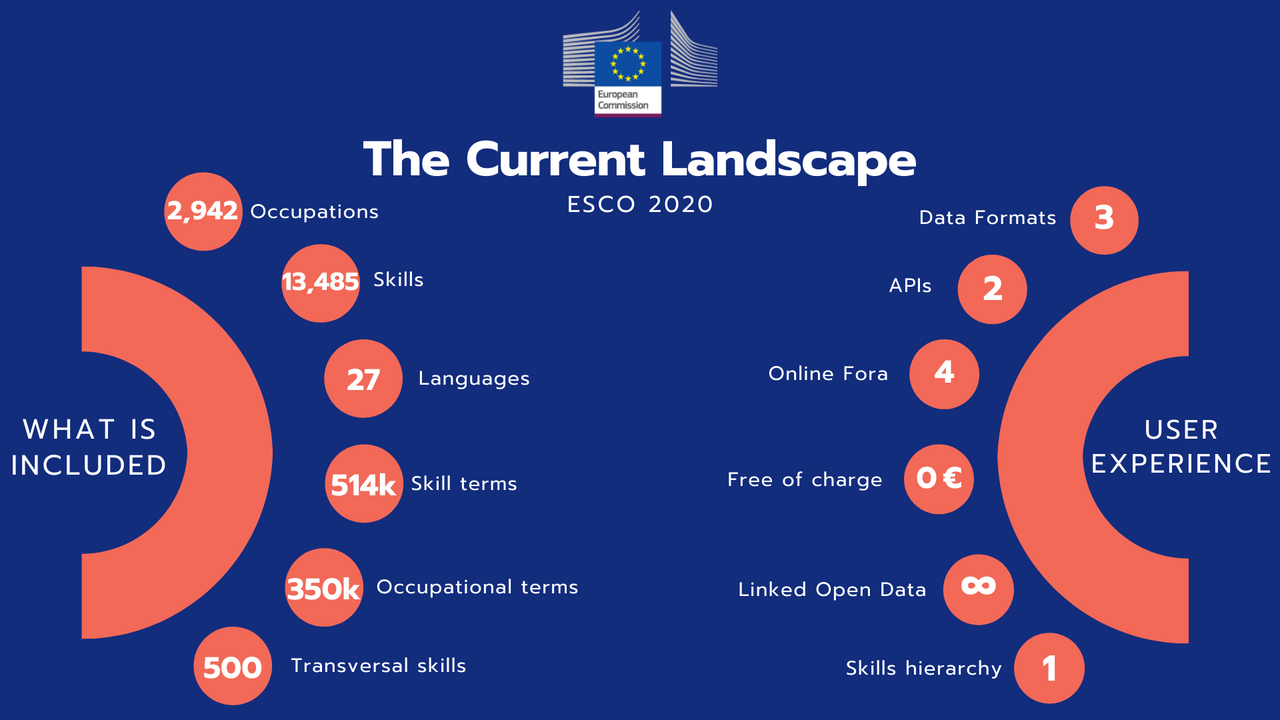
\includegraphics[width=15cm]{figs/ESCO_Landscape.png}
    \caption{\acs{esco}'s Landscape in September 2022 - currently the taxonomy contains information about 3,008 occupations and 13,890 skills~\cite{what_esco}}
    \label{fig:esco_landscape}
\end{figure}

People change jobs and employers more frequently than in the past, new skills are regularly needed while geographic and job mobility increases. Both employers and job seekers are turning more to digital methods for posting and applying for jobs, as well as for seeking and providing training opportunities. Companies and educational institutions need clear and updated information on skills and qualifications to better address skills gaps in education~\cite{esco_needed}.  

Therefore, the aim of \ac{esco} is to support job mobility across Europe and, consequently, achieve a more integrated and efficient labour market, by offering a “common language” on occupations and skills that can be used by different stakeholders on employment, education and training topics~\cite{what_esco}. 

\ac{esco}’s classification can be accessed through two types of APIs, a web-service API, available online, and a Local API which, as the name suggests, needs to be installed locally~\cite{esco_api}.

The \ac{esco} Web Services API is a web-based service that offers access to various versions of the \ac{esco} classification, encompassing functionalities that address most \ac{esco} business use cases. Featuring an easy-to-use web interface for linked data (disposed hierarchically), each concept is identified as an URI, making it a perfect setup for non-technical users. This service allows text search for Occupations, Skills \& Competences and Qualifications.

\begin{figure}[H]
    \centering
    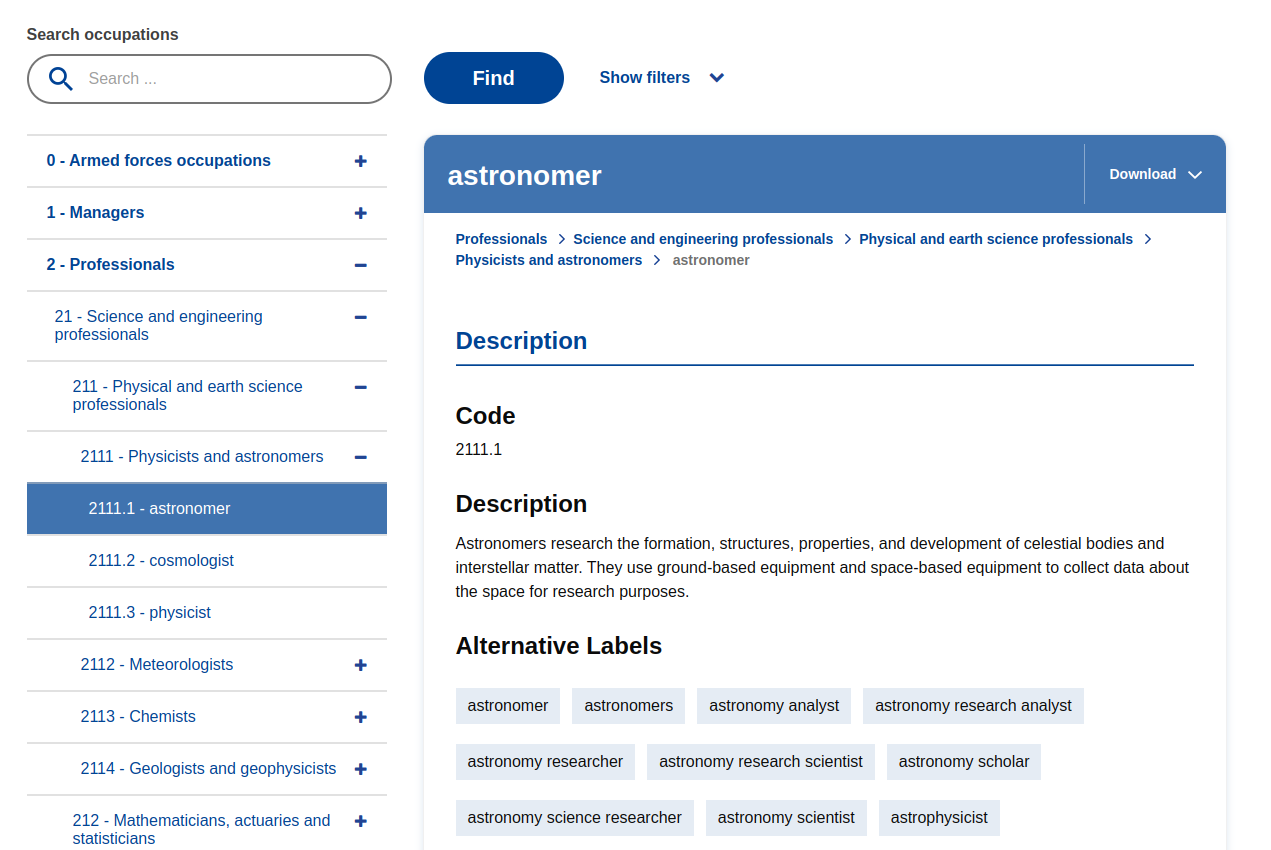
\includegraphics[width=15cm]{figs/esco_web_service.png}
    \caption{Example of an \acs{esco}'s Web Service page~\cite{astronomer}}
    \label{fig:esco_web_service}
\end{figure}

The \ac{esco} Local API is a downloadable version of the \ac{esco} API, which can be installed on a computer or server, providing local access to \ac{esco}’s information. Compared to the Web Services API, this local version assures increased performance and the independence from the availability of the service provided by the European Commission.

\subsection{ISCO}
The \ac{isco} is a globally recognized framework developed by the International Labour Organization (ILO) to categorize and organize occupations~\cite{isco}. Just like \ac{esco}, this taxonomy serves as a vital tool for labour market analysis, providing a standardized system for classifying jobs based on the skills, education, and duties involved. \ac{isco} is structured hierarchically, with major groups divided into sub-major groups, minor groups, and unit groups, each with different levels of detail and specificity. The two latest versions of \ac{isco} are ISCO-88 (dating from 1988) and ISCO-08 (dating from 2008)~\cite{esco_isco_relation}.
\ac{esco} was actually influenced and inspired by \ac{isco}, particularly in its approach to structuring occupations. \ac{esco} maps each occupation to an ISCO-08 code and uses ISCO-08 as a hierarchical structure for its occupations pillar, indicating a direct link and a level of compatibility and interoperability between the two systems~\cite{esco_isco}.

\begin{figure}[H]
    \centering
    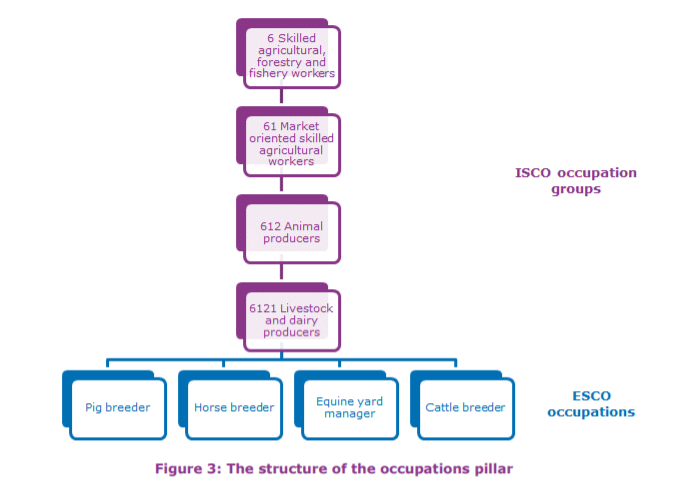
\includegraphics[width=15cm]{figs/esco_isco.png}
    \caption{Role of ISCO-08 in the hierarchical structure of the ESCO occupations pillar~\cite{esco_isco}}
    \label{fig:esco_isco}
\end{figure}


This alignment with ISCO-08 enables \ac{esco} to both:
\begin{itemize}
    \item maintain consistency with a globally recognized occupational classification system, ensuring harmonization with international standards.
    \item enhance its utility for the European labour market - facilitating comprehensive market analysis and mobility across borders.
\end{itemize}


\subsection{O*NET}
\ac{onet} is the American equivalent of \ac{esco}, developed under the sponsorship of the U.S. Department of Labor/Employment and Training Administration (USDOL/ETA)~\cite{esco_onet_crosswalk}, comprising occupations from the Standard Occupational Classification (SOC) system and their corresponding skills, knowledge, and abilities~\cite{Fareri_2021}.
Just like the above taxonomies, \ac{onet} aims to provide a comprehensive database of job characteristics and work skills that standardizes and categorizes the labour market, in this case, of the American panorama.

\begin{figure}[H]
    \centering
    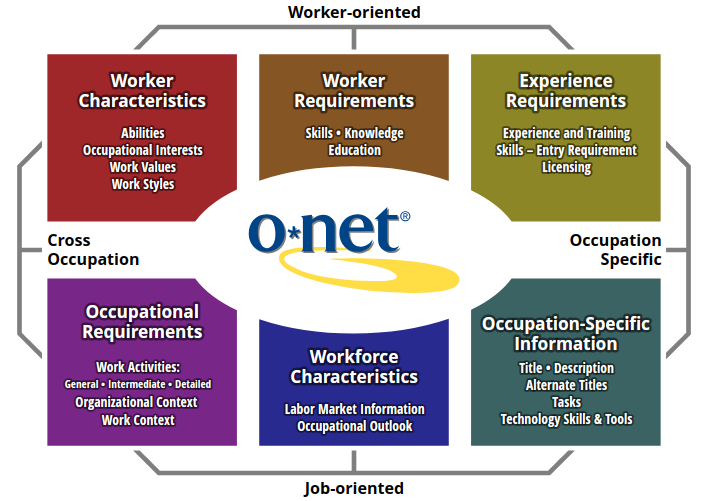
\includegraphics[width=15cm]{figs/onet_content_model.png}
    \caption{The O*NET® Content Model schematic representation~\cite{onet_content}}
    \label{fig:onet_content}
\end{figure}

The \ac{onet} Content Model~\cite{onet_content} serves as the structural foundation for the \ac{onet} database, outlining critical occupational information by integrating job-oriented and worker-oriented descriptors. Developed through job analysis research, it includes six domains that detail attributes and characteristics relevant both across occupations (cross-occupational descriptors) and within specific jobs (occupation-specific descriptors), facilitating a comprehensive understanding of various roles and worker qualities.

According to~\citeauthor{Fareri_2021}, when compared to \ac{esco}, this taxonomy lacks in the level of detail, as the latter possesses six times more skills and three times as many job profiles~\cite{Fareri_2021}.
Furthermore, there was a cooperation between the \ac{esco} Secretariat and the US Department of Labor to develop a crosswalk between the two frameworks~\cite{esco_onet_crosswalk} with the aim to “create a bridge” that supports interoperability between two labour market standards using machine learning models and human validation.

\begin{figure}[H]
    \centering
    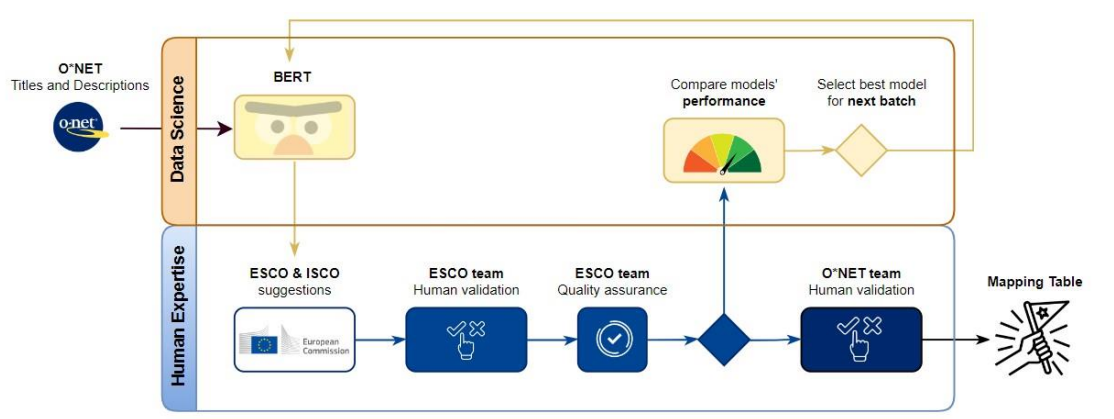
\includegraphics[width=15cm]{figs/crosswalk.png}
    \caption{ESCO-O*NET crosswalk methodology~\cite{esco_onet_crosswalk}}
    \label{fig:crosswalk}
\end{figure}

The European Commission developed AI models (fine-tuned BERT base-uncased) to match \ac{onet} occupations to \ac{esco} occupations based on textual similarity. These models were trained using expert feedback, national taxonomies, qualifications, and job vacancies. The best model suggested ten \ac{esco} occupations for each \ac{onet} occupation, representing the highest semantic similarity. Then, the \ac{esco} team validated these suggestions, distributing the tasks among members and following specific rules to determine the relationship between O*NET-ESCO pairs. The validation process included quality checks and, if necessary, third-party involvement for disagreements. 

This project involved two parallel efforts: iterative improvements by the data science team based on validation feedback and collaboration with the U.S. Department of Labor for further validation and refinement. The final crosswalk table, agreed upon by both teams, is now available on the \ac{esco} Portal.

\section{Large Language Models (LLMs)}
\label{sec:llms}

\ac{llms} consisting of Neural Networks with billions of parameters and trained on vast quantities of unlabeled data (to understand language patterns, grammar and semantics) and labeled data (to guide the model towards more specific tasks)~\cite{lyu2023improving} have significantly impacted the fields of \ac{nlp} and Artificial Intelligence (AI), representing a major transition in how machines understand and generate human language and how they return the information. The history of \ac{llms} is rooted in the development of Machine Learning (ML) and \ac{nlp}, with their emergence being a complete change in the game when it comes to algorithm enhancing, computational power, data availability and data retrieval.

As mentioned, \ac{nlp} has been fundamental to the development and operation of \ac{llms}. Its approach usually involves the execution of a software pipeline with the aim of extracting information from text~\cite{CHIARELLO2021121177}. These approaches have been widely used in different fields, for example, in the analysis of customer reviews, social media usage, patents and, more recently, in the analysis of skill demand and job profiles~\cite{CHIARELLO2021121177, Fareri_2021}.

The field's progression from syntactic analysis to understanding semantics and pragmatics of language has directly influenced the capabilities of these models. \ac{nlp} techniques are crucial in pre-processing data for \ac{llms}, handling tasks like tokenization, part-of-speech tagging, and entity recognition, which are vital for training these models effectively. Furthermore, advances in \ac{nlp} have continually pushed the boundaries of what's possible with \ac{llms}, leading to more sophisticated and context-aware models.

Today, \ac{llms} are an integral part of a wide range of applications. From chatbots and virtual assistants to advanced text generation and translation, they have shown their ability to improve performance on text retrieval tasks through the generation of synthetic training data based on real examples~\cite{clavié2023large}, transforming the way machines interact with human language. 

With the increasing use of \ac{llms}, the concern in developing and optimizing prompts to achieve the best possible answers gave rise to a new discipline, Prompt Engineering~\cite{prompt_engineering}. Prompt engineering is much more than just designing and developing prompts. It gathers a certain set of skills and techniques that enhance the interaction and development with \ac{llms}, allowing for their augmentation with domain knowledge and external tools.

In the context of this work, we will discuss two important techniques of Prompt Engineering, \textbf{Zero-Shot Prompting} and \textbf{Role-Play Prompting}.

In \ac{nlp} and \ac{llms}, Zero-Shot Prompting is understood as providing a prompt to the model that is not part of the training data, but for which the model can provide a desirable result or answer~\cite{zero_few}. This technique relies mainly on the model’s reasoning.

\begin{figure}[H]
    \centering
    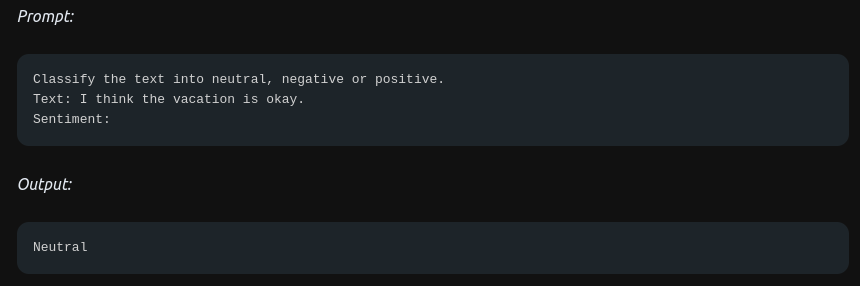
\includegraphics[width=15cm]{figs/zero_shot.png}
    \caption{Example of a Zero-Shot prompt and answer~\cite{zero_shot}}
    \label{fig:zero_shot}
\end{figure}


In Figure \ref{fig:zero_shot} a simple application of \textbf{Zero-Shot Prompting} is represented, where no context or further information is given, just a simple task that tests the model’s reasoning. In the next section, an application of this technique, focused on skills matching, is explored.

Modern \ac{llms}, such as \textit{ChatGPT} and \textit{Google Bard} show an extraordinary capacity for role-playing, being able to not only embody human characters, but also non-human entities, such as the Linux terminal~\cite{kong2023better}. That capacity can be referred to as \textbf{Role-Play Prompting}. This behavior allows the models to simulate complex human-like interactions and perform certain tasks differently, regarding the context prompted and the entity they are embodying. This is a really important feature that can be very useful for this work and will be further discussed in Chapter \ref{chapter:methodology}.

\section{Applying NLP and LLMs to Occupation and Skill Taxonomies}
\label{sec:applying}
As we’ve seen in the previous section, \ac{nlp} and \ac{llms} offer sophisticated tools that can be used to interpret and process text from job descriptions and educational/training offers, helping in mapping their content to \ac{esco} competences, for example.

Therefore, this section will cover various aspects and approaches related to the use of \ac{nlp} and \ac{llms} in the specific context of skill extraction and subsequent alignment with occupational taxonomies, specifically focusing on the matching of these skills to the \ac{esco} framework.


\subsection{Skill-Span Extraction}
\label{sec:skillspan}
The paper~\citetitle{zhang2022skillspan}~\cite{zhang2022skillspan} presents an innovative approach to extract skills from job postings. It roughly consists of a dataset of job postings annotated at the span-level\footnote{A span is a specific, continuous segment of text} for hard and soft skills. Initially, the authors focus on manual annotations by domain experts, to accurately identify specific spans of text that correspond to skills in job postings. This manual annotation is crucial because it will be used to train and fine-tune various BERT models for automatic skill extraction and classification of the manually annotated skill spans. The effectiveness of these models is also explored, highlighting the importance of fine-grained, span-level annotations for a more accurate representation of skills in job postings.

While the final goal of this study is to provide a well-built approach on automated skill extraction, the initial step of dataset creation and annotation relies heavily on human expertise, which is a very lengthy and time-consuming process, especially if we take into account that \ac{esco} contains 13,890 skills. In the following section, a method to fully automate this process is proposed.


\subsection{Zero-Shot Matching}
In~\citetitle{clavié2023large}, the authors explore the application of \ac{llms} in skill matching tasks, particularly mapping job descriptions to \ac{esco} competences. In this approach, a well-thought synthetic data generation is carried out~\cite{clavié2023large}: for each of the 13,890 skills contained in \ac{esco}, they prompted GPT-3.5 to generate forty example sentences that could be used in a job posting in order to refer to the skill. The prompt used for this purpose is provided by the authors in the appendix of the paper.  

Furthermore,~\citeauthor{clavié2023large} propose a two-step process for their skills matching pipeline: initially generating a list of potential matches for a given job description, followed by re-ranking these matches. 
To generate the list of potential matches, the authors use two distinct approaches. The first one relies on simple logistic regression classifiers and the second one is based on cosine similarity between the job description text and the sentences previously generated by GPT-3.5.

In the second phase of the skills matching, \ac{llms} are employed as zero-shot re-rankers (explained in section \ref{sec:llms}~\cite{prompt_engineering}) i.e., without further context, the LLM is prompted to rank the list of potential matches according to their relevance or appropriateness for the job post. 

This approach, requiring no human annotations, significantly outperforms previous methods, highlighting the transformative impact of \ac{llms} in automating and refining the process of mapping complex job descriptions to specific skill sets within a recognized framework, in the case, \ac{esco}.

\begin{figure}[H]
    \centering
    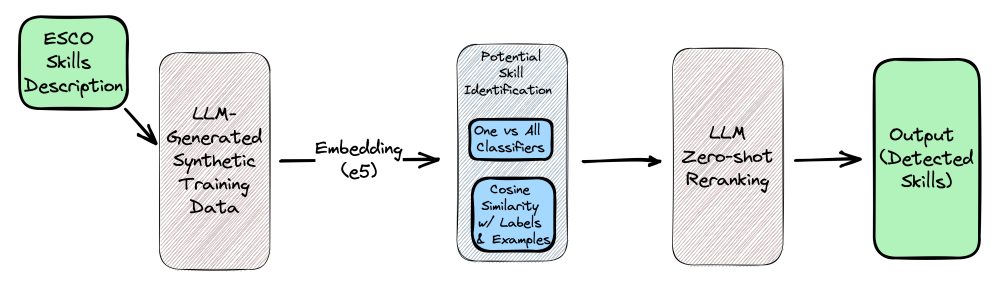
\includegraphics[width=15cm]{figs/zero_shot_process.png}
    \caption{High-level overview of the full Zero-Shot process~\cite{clavié2023large}}
    \label{fig:zero_shot_process}
\end{figure}


\subsection{Distant Supervision}
\label{sec:supervision}
In~\citetitle{zhang2022kompetencer}~\cite{zhang2022kompetencer} and ~\citetitle{decorte2022design}~\cite{decorte2022design} a distinct approach is taken. In these two papers, the authors rely on distant supervision for skill extraction, although with some differences between them. 
“Distant supervision is a technique of labeling data for relation extraction utilizing an existing knowledge database”~\cite{10.1371/journal.pone.0216913}, in this specific context, the database is \ac{esco}.

In~\cite{decorte2022design} the authors use distant supervision to create a training set for skill extraction (Fig. \ref{fig:negative_sampling} - 2). They collect sentences from job vacancies (Fig. \ref{fig:negative_sampling} - 1) that explicitly mention skills of the \ac{esco} taxonomy, a highly precise method that can, however, lead to false negatives. Then, negative sampling strategies are introduced to improve learning (Fig. \ref{fig:negative_sampling} - 3), this consists in “combining ‘positive sentences’ for a given skill (i.e., sentences labeled with that skill during the distant supervision step) with sentences not containing that skill (referred to as ‘negative sentences’)”. Finally, a pre-trained RoBERTa model is used to train binary classifiers for each skill (Fig. \ref{fig:negative_sampling} - 4).

\begin{figure}[H]
    \centering
    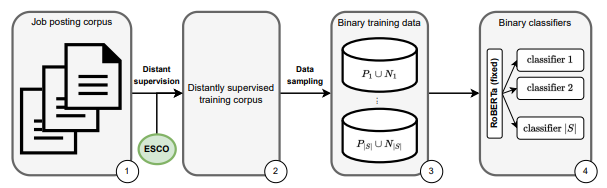
\includegraphics[width=15cm]{figs/negative_sampling.png}
    \caption{Schematic representation of Negative-Sampling processes~\cite{decorte2022design}}
    \label{fig:negative_sampling}
\end{figure}

In~\cite{zhang2022kompetencer}, ~\citeauthor{zhang2022kompetencer} also use distant supervision, in this case, with the \ac{esco} API as reference. The authors annotate a Danish job posting dataset at a span-level, i.e., they identify and label spans within the dataset that correspond to particular skills (following the same logic as explained in the section \ref{sec:skillspan}), while using the \ac{esco} API for distant supervision to obtain fine-grained labels. After that, various BERT models are fine-tuned on the distantly supervised labels and used to classify the spans. Besides that, the authors even presented experiments based on Zero-Shot and Few-Shot Prompting to address the problem of skill extraction.

\begin{figure}[H]
    \centering
    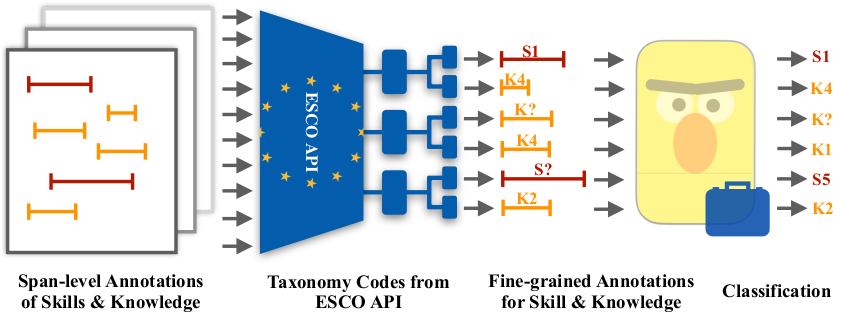
\includegraphics[width=15cm]{figs/kompetencer.png}
    \caption{Pipeline for Fine-grained Danish Skill Classification in Kompetencer~\cite{zhang2022kompetencer}}
    \label{fig:kompetencer}
\end{figure}



For this dissertation work, a mixture of the \textbf{Zero-Shot approach} and the \textbf{Distant Supervision} approach should take place in order to take maximum advantage of both LLM and \ac{esco} API. The data generation method used by~\citeauthor{clavié2023large}~\cite{clavié2023large} could also be adapted for this thesis in order to process all of the \ac{esco} skills, but generating educational offers instead of job postings. However, the other presented approaches will also be taken into account during the implementation of this thesis work, as they provide interesting insights and solutions for different problems.

\chapter{Methodology}
\label{chapter:methodology}

\section{Methodology}
In this chapter, aspects related to the thesis work methodology will be discussed, such as initial approaches, aspects to consider when developing the system, attacks to the problems inspired by the literature review in section \ref{sec:applying}, etc.
Therefore, in order to better understand what is going to be developed, we start by analyzing a small diagram, Figure \ref{fig:diagrama}, that summarizes the interactions and relationships between the different parts involved in the system.

\begin{figure}[H]
   \centering
   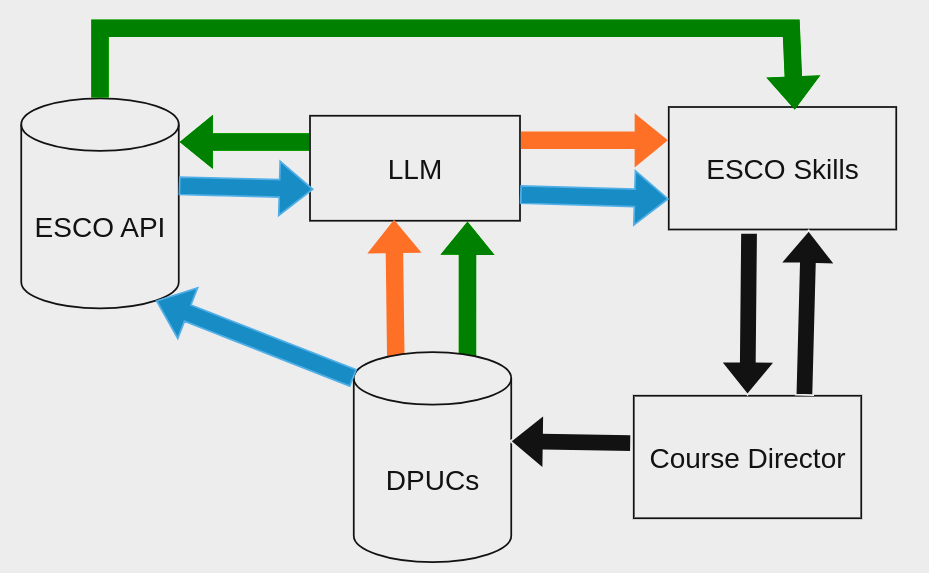
\includegraphics[width=15cm]{figs/diagrama.png}
   \caption{Diagram representing the system's pipeline, with different possible flows}
   \label{fig:diagrama}
\end{figure}

Let's start by explaining what the five entities in the diagram consist of:
\begin{itemize}
   \item \ac{esco} API - explained in section \ref{sec:esco}, it is crucial for the system to work properly, as it is the main source of information for skills matching.
   \item \ac{dpuc} - document containing the detailed information of a specific UA course or micro-credential, the structure of which will be explained further on. UA has a database that contains every \ac{dpuc}
   \item LLM - will be responsible for assisting in the pre and post-processing of data from the \ac{dpuc}s and the \ac{esco} API.
   \item \ac{esco} skills - these are the final product of the system, the aim is for them to be as related to the course or micro-credential in question as possible.
   \item Course Director - professor responsible for managing the \ac{dpuc} of the course for which he/she is responsible (human expert in the matter) and for evaluating the skills determined (i.e. approving or discarding the determined skills based on their similarity to the learning outcomes of the course). 
\end{itemize}



As we can denote, in Figure \ref{fig:diagrama} there are three paths that can be followed, each of which represents a different approach to the system flow.

The \textbf{orange} path represents more of a test than a real possibility for the system's flow. In this approach, the information coming from courses’ \acp{dpuc} is provided directly to a LLM (a few tests were conducted using both \textit{ChatGPT 4}~\cite{chatgpt} and \textit{Google Bard}~\cite{bard}) and it is then prompted to return a list containing the \ac{esco} skills that accurately match the course’s description. Although, since no LLM in the market was trained with \ac{esco} data, the tendency is for these models to hallucinate and give general skills that rarely match the specific \ac{esco} ones.

In the \textbf{blue} path, the information coming from the \acp{dpuc} is provided to the \ac{esco} API in an HTTP query (the process of which will be further on explained). After that, \ac{esco} API returns a list of skills that should match the input of the query. This list is then provided to the LLM alongside with the already mentioned \acs{dpuc} information for post-processing. The skills that do not appropriately match the \acs{dpuc} are discarded, trusting in the model’s ability for this serialization task. This process is repeat for each and every course and micro-credential.

In the \textbf{green} path, \ac{dpuc}’s information is firstly provided to the LLM for pre-processing in order to obtain a list of keywords that appropriately represent the description. This process is conducted so that only crucial information is provided to the \ac{esco} API before the query (acting as a filter). Finally, the query is done to the API to obtain the list of skills.

A combination of both the blue and green path can take place with a double passing through the LLM framework for pre and post-processing, as it could significantly improve the results.

The final step should be the feedback of the Course Directors, assessing the final list of skills for their lecturing course, discarding the skills that do not match the learning outcomes. The Course Directors are also responsible for managing the \ac{dpuc}s of the courses they lecture. Both of these interactions are represented by the black arrows in Figure \ref{fig:diagrama}.

The possibility of using only the \ac{esco} API to match an educational offer to \ac{esco} skills has been set aside since, after some tests, the API has shown itself incapable of returning an accurate set of skills for the provided information (i.e., some of the skills returned were non-sense and in no way related to the educational offer). An email was sent to the \ac{esco} development team, delegated by the European Commission, in order to understand which algorithm or logic was behind the fetching of these skills because it’s not well detailed in the \ac{esco} API documentation~\cite{esco_api_doc}, but no further answer was given to this date.

Before starting the implementation of anything, it is necessary to get acquainted with the \ac{esco} API. For that matter, a careful study and analysis of the API took place.
Afterwards, a \textit{Python} script was created to parse the information of a document that contains every UA \ac{dpuc}, which leads us to explain how they are structured.

A \ac{dpuc} is like an identity card for UA’s courses. It contains many fields that describe the educational offer, such as the contents, the objectives, the learning outcomes, the requirements, the recommended bibliography, how the assessment is done, and so on. Of course, not all of these fields are of interest to us in order to find the list of skills that represent this educational offer so, a decision was made to extract only the \textbf{course title}, \textbf{contents}, \textbf{objectives} and \textbf{learning outcomes} fields from the document.

What about micro-credentials? According to the European Commission, “Micro-credentials certify the learning outcomes of short-term learning experiences, for example a short course or training. They offer a flexible, targeted way to help people develop the knowledge, skills and competences they need for their personal and professional development”~\cite{microcredentials}.

Hopefully, in the eyes of UA's information systems, micro-credentials are seen as a normal course, so the logic for extracting the desired fields is the same.

\begin{figure}[H]
   \centering
   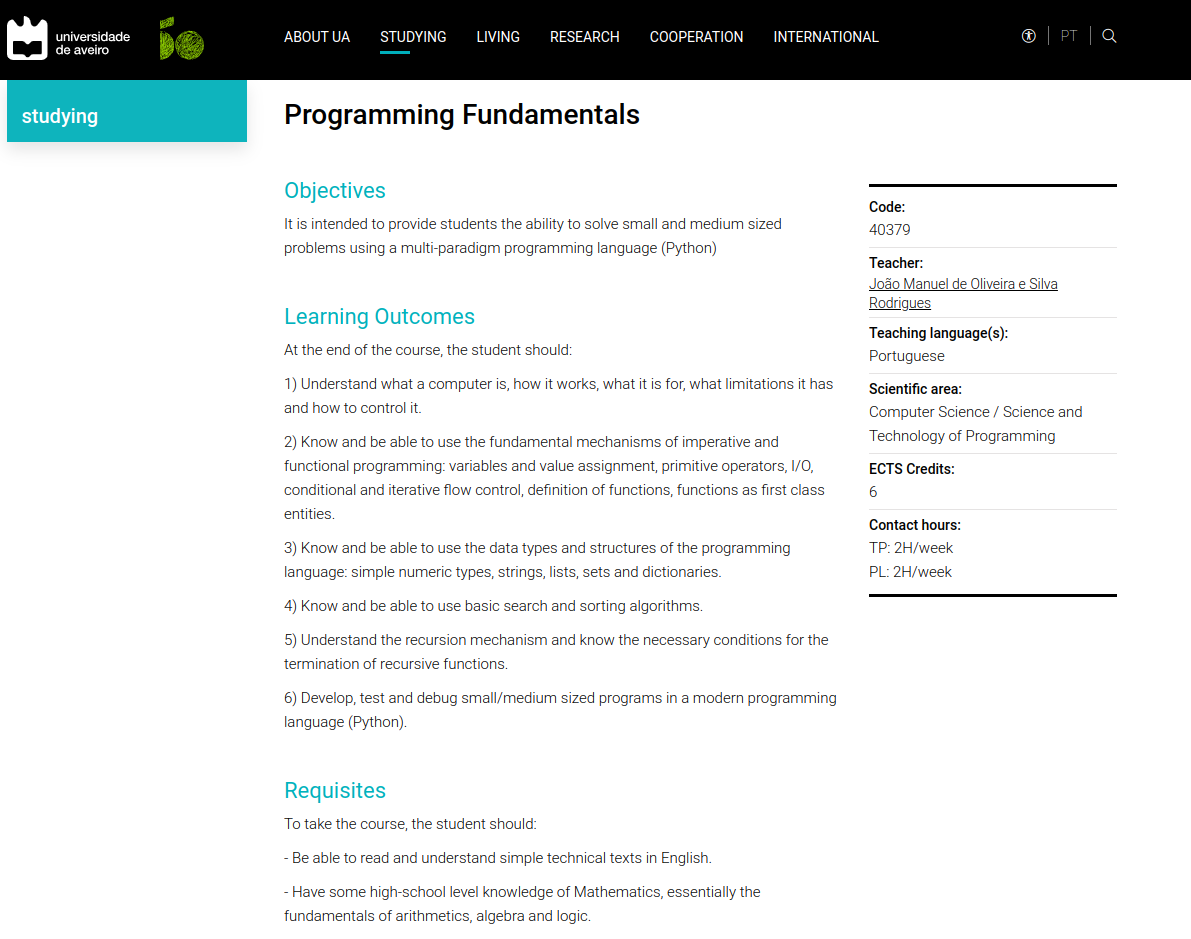
\includegraphics[width=15cm]{figs/dpuc_fp.png}
   \caption{Example of an UA's DPUC web page for the course of Programming Fundamentals~\cite{dpuc}}
   \label{fig:dpuc}
\end{figure}

After obtaining the \ac{dpuc} data for input, it is necessary to find a way to obtain the list of skills. For that purpose, a scholarship student from UA, Lúcia Sousa, that was assigned to an \ac{esco} related project previous to this thesis, developed a script to query the \ac{esco} API and obtain a list of skills for the provided text. At that time, Lúcia was trying to generate a list of skills that could accurately represent the information of UA’s project courses (for example, Project in Informatics, Project in Biomedical Engineering, etc) only using the \ac{esco} API but, as concluded above, she also found out that the API by itself was not capable of returning such a list. Her script uses the HTTP GET endpoint “/search”~\cite{esco_api_doc} and was adapted to fit the needs of this project.

~\citeauthor{zhang2022kompetencer} suggest the using of Levenshtein distance\footnote{Distance given by the minimum number of operations needed to transform one string into the other} to help in finding the best match for a non-\ac{esco} skill in the \ac{esco} API~\cite{zhang2022kompetencer}. This method relies on distant supervision (section \ref{sec:supervision}) and can be successfully integrated in the system’s flow to filter the API’s results. 

The idea of using \ac{llms} for this use case gains more consistency now. As we have already seen, we can use these models for pre and post-processment, in many different ways (section \ref{sec:applying}). The objective was to use a free and open-source LLM. 

After some research, \textit{Google Bard}~\cite{bard} seemed like a perfect fit, not only because it was developed by Google, but also largely due to the fact that the open-source community developed a \textit{Python} package~\cite{bard_api} that returns responses from \textit{Google Bard} through cookie values, which allows for programmatically integration in this thesis’ system.

\textit{Bard} is a conversational generative artificial intelligence chatbot developed by Google, based initially on the LaMDA family of \ac{llms}, later upgraded to PaLM and, more recently, to Gemini~\cite{bard_api}.

The capacity of \textit{Bard} to perform text processing tasks and role-playing, embodying entities such as an HR Representative, a Course Director and a long-life learner allow for a perfect fit in the system’s pipeline, as the prompt’s context can be modeled to achieve more filtered and straight to the point answers.

Even though some advances and experiments have been conducted using \textit{Bard} in this thesis work, the door to other \ac{llms} will always remain open, as they can contribute greatly to a more complete and accurate work.

Finally, when the list of skills is obtained for each UA course and micro-credential, these should be manually reviewed and assessed by the responsible Course Director to assure that every skill correctly matches the educational offer.
This feedback is extremely important to evaluate the system's performance.

%%%%%%%%%%%%%%%%%%%%%%%%%%%%%%%%%%%%%%%%%%%%%%%%%%%%%%%
% End of Thesis text 
%%%%%%%%%%%%%%%%%%%%%%%%%%%%%%%%%%%%%%%%%%%%%%%%%%%%%%%

\backmatter

%%%%%%%%%%%%%%%%%%%%%%%%%%%%%%%%%%%%%%%%%%%%%%%%%%%%%%%
% Print all used references
%%%%%%%%%%%%%%%%%%%%%%%%%%%%%%%%%%%%%%%%%%%%%%%%%%%%%%%

\begingroup
\renewcommand{\bibfont}{\footnotesize}
% Redefine References name to Portuguese
% Change if you are using english
\defbibheading{bibliography}[References]{
	\chapter{#1}
}
\SingleSpacing
\setlength\bibitemsep{8pt}
\printbibliography[heading=bibliography]
\endgroup


%%%%%%%%%%%%%%%%%%%%%%%%%%%%%%%%%%%%%%%%%%%%%%%%%%%%%%%
% Load appendix
%%%%%%%%%%%%%%%%%%%%%%%%%%%%%%%%%%%%%%%%%%%%%%%%%%%%%%%

\mainmatterWithoutReset
\appendix

% \include{appendix-a}
% \include{appendix-b}
% \include{appendix-c}
\chapter{Additional content}

\end{document}